\section{Overordnet kravspecifikation}
Systemet afspejler det system TV2 har lagt op til i projekt-casen. Der er tale om et system, hvor man kan se - og redigere krediteringer for programmer. Systemet skal kunne tilgås via en dansk brugergrænseflade. Det skal indeholde forskellige brugerroller; Administrator, bruger og gæst. Producere der kan tilføje og redigere i krediteringerne, skal kun have mulighed for at redigere i de produktioner, de selv ejer.\\

\noindent
Kanaladministratoren skal kunne redigere, oprette og slette krediteringer for et givent program. En bruger skal kunne redigere samt oprette krediteringer for et givent program, og en gæst skal kunne se krediteringer for alle programmer. Det skal være muligt at kombinere personer som refererer til den samme person i den virkelige verden. Når to forskellige producere vil oprette en kreditering for et program, skal krediteringen være associeret med en person og vedkommendes rolle. Det betyder altså, at det skal være muligt at oprette personer der kan sammenflettes (f.eks. med UUID).\\

\noindent
TV2 har ikke lov til at lagre persondata, såsom et CPR-nummer eller et telefonnummer, så det skal være muligt at identificere personer i systemet og sikre at krediteringerne er korrekt forbundet til de rigtige personer.
Det skal være muligt at eksportere en specifik mængde data i forskellige formater såsom XML og CSV. Derudover skal databasen være søgbar, så det er nemt at finde personer, programmer og lignende. Det er vigtigt at systemet er nemt at bruge, så seerne nemt kan se krediteringerne for det program de lige har set.\\

\noindent
TV 2 kunne være interesseret i at integrere systemet med andre systemer (Yousee Play, Boxer play osv.), og det er derfor vigtigt at systemet er kompatibelt med krediteringer i andre systemer. Det kunne også være interessant at have muligheden for at få notifikationer når noget nyt sker i systemet. Samrådet for Ophavsret og Producentforeningen kunne også være interesseret i at modtage en form for meddelelse hver gang der er blevet tilføjet noget nyt til systemet, hvor de kan godkende krediteringerne og ud fra disse udbetalte royalties.\\

\noindent
For at beskytte dele af systemet (tilføjelse/redigering/sletning af data osv.), skal der indføres en form for adgangskontrol. Der skal være en offentligt tilgængelig del af systemet, hvor det er muligt at se krediteringerne for et et program uden at skulle logge ind.
\begin{center}
\begin{table}
\begin{tabular}{ |p{1cm}|p{3.5cm}|p{7cm}| }
\hline
\textbf{ID} & \textbf{Navn} & \textbf{Beskrivelse} \\
\hline
K01 & Brugergrænseflade & Systemet skal tilgås via en dansk brugergrænseflade \\
\hline
K02 & Brugerroller & Systemet skal indeholde brugerroller \\
\hline
\label{K03}K03 & Tildel roller & Kanaladministrator skal kunne tildele producer- og kanaladministrator roller \\
\hline
K04 & Slet bruger & Systemadministratoren skal kunne slette brugere \\
\hline
K05 & Se krediteringer & Alle skal kunne se krediteringer \\
\hline
K06 & Søg efter krediteringer & Alle skal kunne søge efter og se krediteringer for alle programmer \\
\hline
K07 & Opret krediteringer & Specielle brugere, kanaladministratore og systemadmin skal kunne oprette
krediteringer for et givent program \\
\hline
K08 & Rediger krediteringer & Specielle brugere, kanaladmin og systemadmin skal kunne redigere krediteringer for egne programmer \\
\hline
K09 & Slet kreditering & Kanaladmin og systemadmin skal kunne oprette/redigere/slette krediteringer under egen kanal \\
\hline
K10 & Søg efter personer & Alle skal kunne søge efter personer \\
\hline
K11 & Knyt personer til krediteringer & Personer skal kunne knyttes til krediteringer så man kan se hvilke programmer en person har deltaget i Systemadmin, kanaladmin og producer skal kunne se persondata som email og tlf. nr. \\
\hline
K12 & Link personer i den virkelige verden & Det skal være muligt at linke personer i krediteringer til personer i den virkelige verden, så der krediteres korrekt \\
\hline
K13 & Eksporter data & Brugere skal kunne eksportere data til forskellige formater såsom XML og CSV \\
\hline
K14 & Importering af data & Systemet skal kunne importere EPG data via TVTid.dk \\
\hline
\end{tabular} 
\caption{Funktionskrav}
\label{table:funktionskrav}
\end{table}
\end{center}

\subsection{Aktørliste}

\scalebox{0.7}{
\begin{center}

\begin{tabular}{ |p{6cm}|p{6cm}|p{6cm}| }
\hline
\textbf{Aktør} & \textbf{Beskrivelse} & \textbf{Mål og tjenester} \\
\hline
Systemadministrator (p) 
& Står for at slette personer \newline Kan søge efter program, kreditering og person information 
& At læse krediteringer, personer og brugere \newline At slette personer \newline Søge efter information \newline Log ind og af \newline Se alt hvad en person har været med i\\

\hline
Kanaladministrator (p) 
& Skal godkende nyoprettede krediteringer \newline Kan slette krediteringer under egen kanal \newline Kan tildele producer- og kanaladministratorroller for egen kanal  
& Ingenting\\

\hline
Royal bruger (p) 
& Kan se persondata, eksportere data samt bekræfte at de har tildelt royalty \newline Kan se krediteringer for forskellige programmer \newline Kan søge efter program, kreditering og person information
& Kan se persondata \newline Kan eksportere data \newline Kan bekræfte når royalties er tildelt \newline Kan se krediteringer for forskellige programmer \newline Søge efter information \\

\hline
Producer (p) 
& Kan bruge systemet til at se krediteringer for forskellige programmer. \newline Har mulighed for at oprette nye krediteringer samt rette krediteringer for egne produktioner. \newline Kan søge efter program, kreditering og person information. \newline Kan trykke på en person og se alt hvad vedkommende har været med i.
& Kan se krediteringer for forskellige programmer \newline Kan søge efter krediteringer for forskellige programmer \newline Kan oprette krediteringer \newline Kan redigere i eksisterende krediteringer for egne produktioner \newline Søge efter information \newline Log ind og af \newline Se alt hvad en person har været med i \\

\hline
Gæst (p) 
& Offentligheden skal kunne finde informationer og krediteringer om forskellige programmer samt personer. \newline Kan søge efter program, kreditering og person information. \newline Kan trykke på en person og se alt hvad vedkommende har været med i.
& Kan se krediteringer for forskellige programmer \newline Kan søge efter krediteringer for forskellige programmer \newline Se alt hvad en person har været med i \newline Søge efter information\\

\hline

\end{tabular}
\caption{Aktørlisten}
\label{table:aktørlist}
\end{center}}

\subsection{Overordnet brugsmønstermodel}
\begin{figure}[H]
\centering 
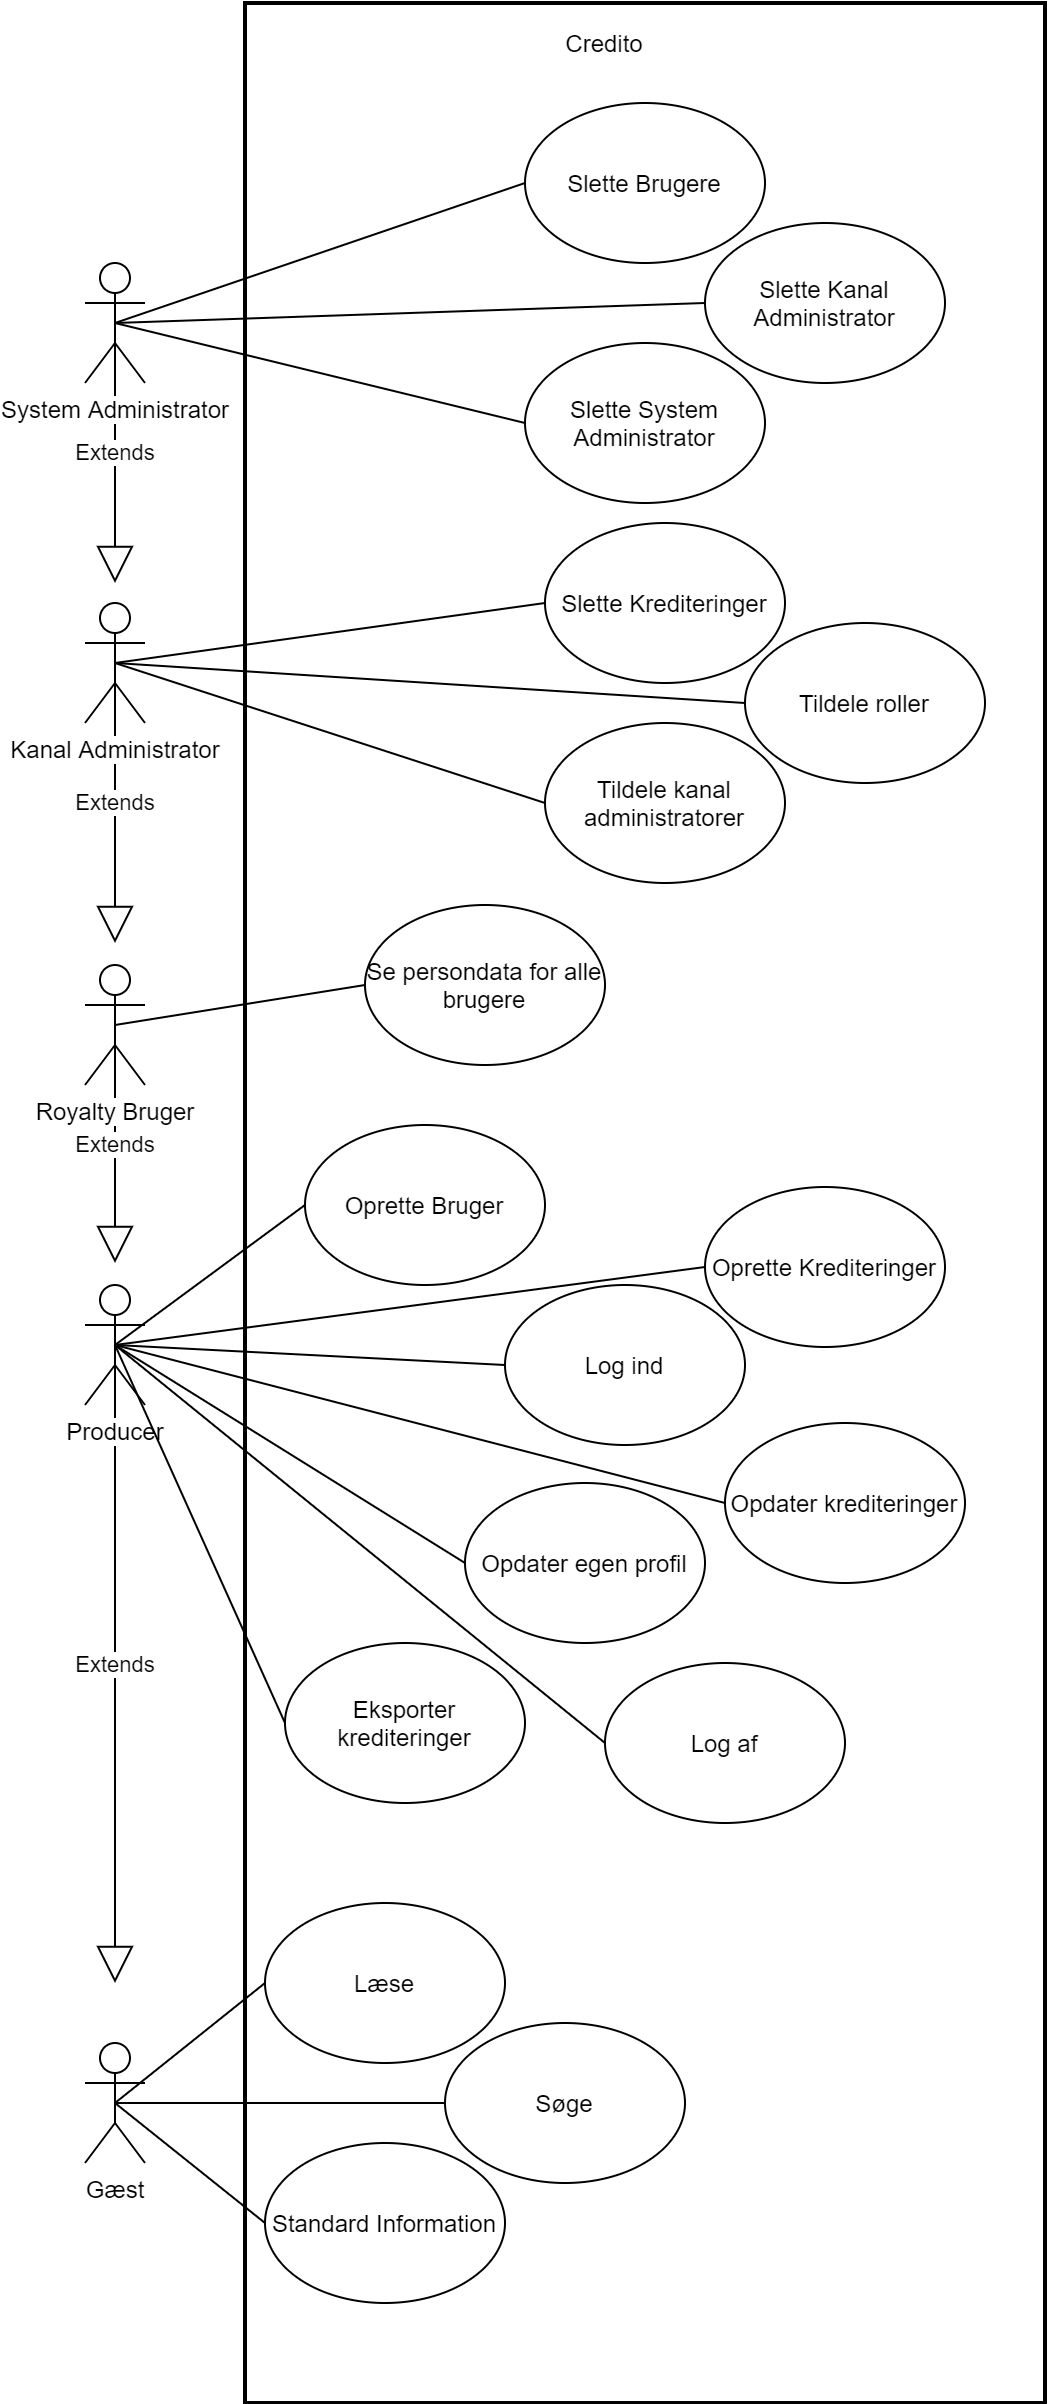
\includegraphics[scale=0.22]{figures/use-case.png}
\caption{Brugsmønster over Creditoro systemet}
\end{figure}

\subsection{Liste over brugsmønstre}
% Det burde nok være en long table?

\begin{table}[H]
\centering
\scalebox{0.9}{
\begin{tabular}{ |p{1cm}|p{3.5cm}|p{10cm}| }
\hline
ID & Navn & Aktør \\
\hline
B01 & Opdater egen royal bruger & Systemadministrator (p), Royal Bruger (p) \\
\hline
B02 & Opdater person & Systemadministrator (p), kanaladministrator (p), producer (p) \\
\hline
B03 & Opret Producer & Systemadministrator (p), kanaladministrator (p) \\
\hline
B04 & Opret person & Systemadministrator (p), kanaladministrator (p), Producer (p) \\
\hline
B05 & Fjern producer & Systemadministrator (p) \\
\hline
B06 & Fjern person & Systemadministrator (p) \\
\hline
B07 & Opret kreditering & Systemadministrator (p), Kanaladministrator (p), producer (p) \\
\hline
B08 & Fjern kreditering til program & Systemadministrator (p), kanaladministrator (p) \\
\hline
B09 & Opdater egne kreditering & Systemadministrator (p), kanaladministrator (p), Producer (p) \\
\hline
B10 & Læse krediteringer & Systemadministrator (p), kanaladministrator (p), Royal Bruger (p), Producer (p), Gæst (p) \\
\hline
B11 & Se person profil & Systemadministrator (p), kanaladministrator (p), Royal bruger (p), Producer (p), Gæst (p) \\
\hline
B12 & Søge efter personer og programmer & Systemadministrator (p), kanaladministrator (p), Royal Bruger (p), Producer (p), Gæst (p) \\
\hline
B13 & Log ind & Systemadministrator (p), kanaladministrator (p), Royal Bruger (p), Producer (p) \\
\hline
B14 & Log af & Systemadministrator (p), kanaladministrator (p), Royal Bruger(p), Producer (p) \\
\hline
B15 & Kan se personinformation & Systemadministrator (p), kanaladministrator (p), Royal Bruger (p), Producer (p) \\
\hline
B16 & Godkende nye krediteringer & Systemadministrator (p), Kanaladministrator (p) \\
\hline
B17 & Afvise nye krediteringer & Systemadministrator (p), Kanaladministrator (p) \\
\hline
B18 & Opret kanaladministrator & Systemadministrator (p), kanaladministrator (p) \\
\hline
B19 & Opret systemadministrator & Systemadministrator (p) \\
\hline
B20 & Bekræfte betalt royalty & Royal Bruger (p) \\
\hline
\end{tabular}}
\end{table}


\subsection{Overordnet supplerende krav}
\begin{table}[H]
\centering
\begin{tabular}{ |p{2cm}|p{2.5cm}|p{7cm}| }
\hline
\textbf{ID} & \textbf{Type} & \textbf{Beskrivelse} \\
\hline
S01 & Notifikationer & Systemet skal give notifikationer til Royal Bruger (p) \\
\hline
S02 & Integration & Systemet skal kunne integreres med andre systemer (YouSee Play, Boxer Play, osv) - Via importering af eksisterende krediteringsdata \\
\hline
S03 & Sprogvalg & Systemet skal understøtte flere sprog \\ 
\hline
\end{tabular}
\caption{Supplerende krav}
\label{table:1}
\end{table}




\subsection{Detaljerede brugsmønstre}

\begin{table}[H]
\begin{tabular}{|p{14cm}|}
\hline
    \begin{center}{}
    \textbf{Brugsmønster:} Opret kreditering  
    \end{center} \\ \hline
    
	\textbf{ID:} UC01 \\ \hline
	\textbf{Primære aktører:} Systemadministrator, kanaladministrator, Producer \\ \hline
	\textbf{Sekundære aktører:} \\ \hline
	\textbf{Kort beskrivelse:} Produceren opretter en kreditering. Heri angives alle der har bidraget til produceringen af TV-programmet, filmen el. lign. \\ \hline
	\textbf{Prækonditioner (Pre conditions):} \\
Aktøren skal være logget på systemet \\ \hline
\textbf{Hovedhændelsesforløb (main flow):} \\
	1. Brugsmønstret starter når en administrator eller producer vil oprette en kreditering \\
	2. Aktøren trykker på knappen ‘Opret Kreditering’ \\
	3. Systemet checker aktørens rolle \\
	4. Aktøren er forbundet til en kanal, og angiver programmets titel \\
	5. Systemet checker om der allerede findes et program med den angivne \\ titel
	6. Aktøren krediterer alle der har medvirket i produktionen af \\ programmet
	7. Aktøren sender den færdige kreditering videre til godkendelse \\
	8. Postkonditioner (post conditions): \\
	9. En kreditering er blevet oprettet \\ \hline
	\textbf{Alternative hændelsesforløb (alternative flow):} \\
Step *: Aktøren kan til enhver tid afbryde oprettelsen af krediteringen \\
Step 4: Hvis aktøren er systemadministrator, er vedkommende ikke forbundet til en kanal, og kan skifte hvilken kanal krediteringen skal oprettes ved. \\

Step 5: Hvis programmets titel allerede eksistere, gøres aktøren opmærksom på dette. \\

Step 8: Hvis krediteringen afvises, laves de fornødne ændringer, og den nye kreditering sendes videre til godkendelse. \\
\\ \hline
\end{tabular}{}
\end{table}

\begin{table}[H]
\begin{tabular}{|p{14cm}|}
\hline
    \begin{center}{}
    \textbf{Brugsmønster:}  Læs kreditering  
    \end{center} \\ \hline
    
	\textbf{ID:} UC01 \\ \hline
	\textbf{Primære aktører:} Systemadministrator, kanaladministrator, producer, royal bruger, gæst \\ \hline
	\textbf{Sekundære aktører:} \\ \hline
	\textbf{Kort beskrivelse:} Alle skal kunne se krediteringen for programmerne. \\ \hline
	\textbf{Prækonditioner (Pre conditions):} \\ \hline
\textbf{Hovedhændelsesforløb (main flow):} \\
1. Brugsmønstret starter når en aktør vil se kredit for et program \\
2. Aktøren søger efter programmet \\
3. Aktøren trykker på det ønskede program \\
4. Systemet checker hvilken rolle aktøren har \\
5. Aktøren bliver omdirigeret til den passende visning af krediteringen \\ \hline
    \textbf{	Postkonditioner (post conditions):} \\
    En kreditering bliver vist \\ \hline

	\textbf{Alternative hændelsesforløb (alternative flow):} \\
Step 2: Hvis programmet ikke findes, får vedkommende besked om at programmet ikke findes 
\\ \hline
\end{tabular}{}
\end{table}
